\tikzset{every picture/.style={line width=0.75pt}} %set default line width to 0.75pt        

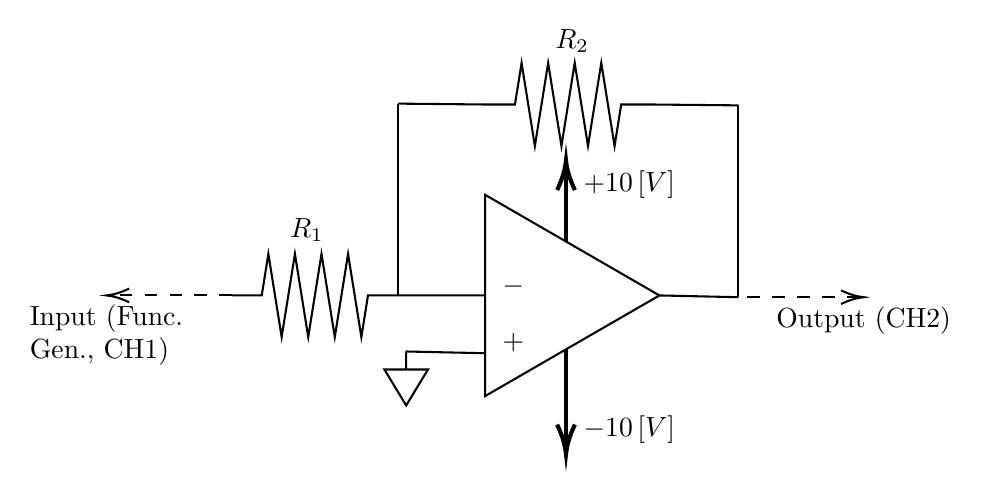
\begin{tikzpicture}[x=0.75pt,y=0.75pt,yscale=-1,xscale=1]
%uncomment if require: \path (0,692); %set diagram left start at 0, and has height of 692

%Straight Lines [id:da973909063029269] 
\draw [line width=1.5]    (290,128.5) -- (290,263.92) ;
\draw [shift={(290,266.92)}, rotate = 270] [color={rgb, 255:red, 0; green, 0; blue, 0 }  ][line width=1.5]    (14.21,-4.28) .. controls (9.04,-1.82) and (4.3,-0.39) .. (0,0) .. controls (4.3,0.39) and (9.04,1.82) .. (14.21,4.28)   ;
\draw [shift={(290,125.5)}, rotate = 90] [color={rgb, 255:red, 0; green, 0; blue, 0 }  ][line width=1.5]    (14.21,-4.28) .. controls (9.04,-1.82) and (4.3,-0.39) .. (0,0) .. controls (4.3,0.39) and (9.04,1.82) .. (14.21,4.28)   ;
%Shape: Ground [id:dp6218025584098273] 
\draw  [fill={rgb, 255:red, 255; green, 255; blue, 255 }  ,fill opacity=1 ] (251,239) -- (335,190.5) -- (251,142) -- (251,239) -- cycle (209,190.5) -- (251,190.5) ;
%Shape: Resistor [id:dp7473730779266806] 
\draw   (129,190.5) -- (143.4,190.5) -- (146.6,170.5) -- (153,210.5) -- (159.4,170.5) -- (165.8,210.5) -- (172.2,170.5) -- (178.6,210.5) -- (185,170.5) -- (191.4,210.5) -- (194.6,190.5) -- (209,190.5) ;
%Straight Lines [id:da4912524923696384] 
\draw    (209,98.08) -- (209,190.5) ;
%Shape: Resistor [id:dp19057956295703093] 
\draw   (251,98.5) -- (265.4,98.5) -- (268.6,78.5) -- (275,118.5) -- (281.4,78.5) -- (287.8,118.5) -- (294.2,78.5) -- (300.6,118.5) -- (307,78.5) -- (313.4,118.5) -- (316.6,98.5) -- (331,98.5) ;
%Straight Lines [id:da44525050708783065] 
\draw    (209,98.08) -- (251,98.5) ;
%Straight Lines [id:da39453577617402236] 
\draw    (331,98.5) -- (373,98.92) ;
%Straight Lines [id:da058156514264413595] 
\draw    (373,98.92) -- (373,191.34) ;
%Straight Lines [id:da29349435917566447] 
\draw    (335,190.5) -- (373,191.34) ;
%Straight Lines [id:da1556742012077138] 
\draw    (213,217.5) -- (251,218.34) ;
%Shape: Ground [id:dp283570639000989] 
\draw   (202.5,226.17) -- (213,243.5) -- (223.5,226.17) -- (202.5,226.17) -- cycle (213,217.5) -- (213,226.17) ;
%Straight Lines [id:da04414817847417474] 
\draw  [dash pattern={on 4.5pt off 4.5pt}]  (129,190.5) -- (70.58,190.5) ;
\draw [shift={(68.58,190.5)}, rotate = 360] [color={rgb, 255:red, 0; green, 0; blue, 0 }  ][line width=0.75]    (10.93,-3.29) .. controls (6.95,-1.4) and (3.31,-0.3) .. (0,0) .. controls (3.31,0.3) and (6.95,1.4) .. (10.93,3.29)   ;
%Straight Lines [id:da6380422554026496] 
\draw  [dash pattern={on 4.5pt off 4.5pt}]  (431.42,191.34) -- (373,191.34) ;
\draw [shift={(433.42,191.34)}, rotate = 180] [color={rgb, 255:red, 0; green, 0; blue, 0 }  ][line width=0.75]    (10.93,-3.29) .. controls (6.95,-1.4) and (3.31,-0.3) .. (0,0) .. controls (3.31,0.3) and (6.95,1.4) .. (10.93,3.29)   ;

% Text Node
\draw (155.6,166.1) node [anchor=south west] [inner sep=0.75pt]    {$R_{1}$};
% Text Node
\draw (283.4,75.1) node [anchor=south west] [inner sep=0.75pt]    {$R_{2}$};
% Text Node
\draw (258,180.4) node [anchor=north west][inner sep=0.75pt]    {$-$};
% Text Node
\draw (258,207.4) node [anchor=north west][inner sep=0.75pt]    {$+$};
% Text Node
\draw (297,128.9) node [anchor=north west][inner sep=0.75pt]    {$+10\left[\text{V}\right]$};
% Text Node
\draw (297,263.52) node [anchor=south west] [inner sep=0.75pt]    {$-10\left[\text{V}\right]$};
% Text Node
\draw (68.58,193.5) node [anchor=north] [inner sep=0.75pt]   [align=left] {Input (Func. \\Gen., CH1)};
% Text Node
\draw (433.42,194.34) node [anchor=north] [inner sep=0.75pt]   [align=left] {Output (CH2)};


\end{tikzpicture}
